\section{Input data} \label{sec:inputdata}

Input data to our network are images in a form of FITS files. Each image contains only one astronomical object as depicted in the Figure \ref{fig:fitsreal3}. The size of the image is 50x50 pixels, as it was mentioned in \cite{Andreon2000} that it is the optimal size of the image for one object to be classified. 
Pixel values of the image are stored in 16 bits, which means that values range from 0 to 65 535. Although the images are in FITS format, we are only making use of the data block and the header is empty. 

In our work, we are using synthetic images as well as real ones. 
However, real images provided by the telescope in AGO have a resolution of 1024x1024 and capture the whole starfield. For us to be able to use these images, we needed to manually cut out 50x50 windows from them with just one astronomical object present. Some examples of such cutouts are shown in the Figure \ref{fig:fitsreal3}.  


\begin{figure}[!h]
   \centering
    \begin{subfigure}{.2\textwidth}
        \centering
        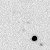
\includegraphics[width=\textwidth]{images/point.png}
        \label{fig:fitsreal3a}
        \caption{Point.}
    \end{subfigure}
    %\hfill
    \begin{subfigure}{.2\textwidth}
        \centering
        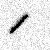
\includegraphics[width=\textwidth]{images/line2.png}
        \label{fig:fitsreal3b}
        \caption{Streak.}
    \end{subfigure}
    %\hfill
    \begin{subfigure}{.2\textwidth}
        \centering
        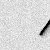
\includegraphics[width=\textwidth]{images/cutline.png}
        \label{fig:fitsreal3c}
        \caption{Cut Streak.}
    \end{subfigure}
    %\hfill
    
    \vspace*{4mm}
    
    \begin{subfigure}{.2\textwidth}
        \centering
        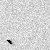
\includegraphics[width=\textwidth]{images/cosmicray.png}
        \label{fig:fitsreal3d}
        \caption{Cosmic ray.}
    \end{subfigure}
    %\hfill
    \begin{subfigure}{.2\textwidth}
        \centering
        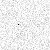
\includegraphics[width=\textwidth]{images/hotpixel.png}
        \label{fig:fitsreal3e}
        \caption{Hot pixel.}
    \end{subfigure}
    %\hfill
    \begin{subfigure}{.2\textwidth}
        \centering
        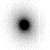
\includegraphics[width=\textwidth]{images/galaxy.png}
        \label{fig:fitsreal3f}
        \caption{Galaxy.}
    \end{subfigure}
    %\hfill
    \caption{Examples of 50x50 pixel cutouts from real images.}
    \label{fig:fitsreal3}
\end{figure}
